\documentclass[letterpaper,openright,12pt,openany]{book}

\usepackage{comment}

%\usepackage[latin1]{inputenc}

\usepackage{ marvosym }

%\usepackage{bold-extra}
\usepackage[utf8]{inputenc} %Permite acentos y demás símbolos directamente
\usepackage[a4paper,includeall,bindingoffset=0cm,margin=2.5cm,
            marginparsep=0cm,marginparwidth=0cm]{geometry}
            
\usepackage{setspace} 
	\setstretch{1.25}
\usepackage{graphicx} %figuras
\usepackage{subfigure} %subfiguras
\graphicspath{{../imagenes/}} % Localización de las carpetas de imágenes

\usepackage{booktabs} % Top and bottom rules for table
\usepackage{multirow} % Permite unir celdas de tablas
\usepackage{rotating}
\usepackage[font=small,labelfont=bf]{caption} % Requerido para especificar descripción de tablas y figuras 
\usepackage{wrapfig} % Permite ajustar texto al rededor de tablas y figuras
\usepackage{longtable} % para tablas largas
\usepackage{float} % para que las gráficas estén donde quiero
\usepackage{changepage} %para cambiar margenes

\usepackage{tikz}
\usetikzlibrary{shapes,arrows}
\usepackage{amsmath}% Para partir ecuaciones 
\usepackage{amsfonts}%Números reales
\usepackage{ amssymb }%Símbolo ángulo

\usepackage{mathtools}

\usepackage[spanish,es-nodecimaldot]{babel}%para usar puntos como separación decimal

\usepackage{afterpage}%Para agregar páginas en blanco
\newcommand{\RomanNumeralCaps}[1]%Para escribir números en romano mayúsculos
    {\MakeUppercase{\romannumeral #1}}
\setcounter{secnumdepth}{4}
\setcounter{tocdepth}{4} % para que añadir las secciones en el índice...


\begin{document}
\pagenumbering{Roman}
    \begin{titlepage}
       \thispagestyle{empty}
        \begin{minipage}[c][0.17\textheight][c]{0.25\textwidth}
            \begin{center}
                \includegraphics[width=3.5cm, height=3.8cm]{unam}
            \end{center}
        \end{minipage}
        \begin{minipage}[c][0.17\textheight][t]{0.65\textwidth}
            \begin{center}
                \vspace{.3cm}
                \textsc{\large Universidad Nacional Autónoma de México}\\[0.5cm]
                \vspace{.1cm}
                \hrule height2.5pt
                \vspace{.1cm}
                \hrule height1pt
                \vspace{.8cm}
                \textsc{\LARGE Facultad de Ciencias}\\[0.8cm] %
            \end{center}
        \end{minipage}

     \begin{minipage}[c][0.81\textheight][t]{0.25\textwidth}
        \vspace*{5mm}
        \begin{center}
            %\hskip1mm
            \vrule width1pt height14cm 
            \hskip9pt
            \vrule width2.5pt height14cm
            \hskip9pt
            \vrule width1pt height14cm \\
            \vskip5mm
            \includegraphics[width=3.8cm, height=4.1cm]{escudoFC}
        \end{center}
    \end{minipage}
    \begin{minipage}[c][0.81\textheight][t]{0.65\textwidth}
        \begin{center}
                \vspace{1cm}

                \LARGE Estudio de tendencias académicas mediante estadística inferencial \\[1cm]

                \vspace{0.8cm}            

                \textsc{\Huge T E S I S}\\[1.8cm]
                \textsc{\large que para obtener el título de}\\[0.7cm]
                \large Matemátio\\[0.7cm]
                \textsc{\large p r e s e n t a}\\[0.7cm]
                \large {Tabaré Merino Sánchez}\\[0.7cm]          

                \textsc{\large Director de tesis:}\\[0.7cm] 
                \large Dr. Miguel Alcubierre Moya\\[1.3cm]

                %\vspace{0.8cm}

                {Ciudad Universitaria, Ciudad de México, 2026}
            \end{center}
            
        \end{minipage}
        \afterpage{\null\newpage}
    \end{titlepage}
\renewcommand{\tablename}{Tabla}

\begin{enumerate}
    \item Datos del alumno
    
	Merino 
	\vspace{-2mm}
	
	Sánchez 
	\vspace{-2mm}
	
	Tabaré
	\vspace{-2mm}
	
	7771591426
	\vspace{-2mm}
	
	Universidad Nacional Autónoma de México
	\vspace{-2mm}
	
	Facultad de Ciencias
	\vspace{-2mm}
	
	Matemáticas
	\vspace{-2mm}
	
	3822437
	
	\item Datos del tutor
	
	Dr
	\vspace{-2mm}
	
	Alcubierre
	\vspace{-2mm}
	
	Moya
	\vspace{-2mm}
	
	Miguel
	
\end{enumerate}

\afterpage{\null\newpage}
\tableofcontents % indice de contenidos

\setlength{\parskip}{1.5mm} % espacio entre párrafos
\pagebreak

\chapter*{Agradecimientos}

\textit{Por último, a cualquier persona que se tome el tiempo de leer mi trabajo. }
\afterpage{\null\newpage}

\pagenumbering{arabic}
\chapter*{Resumen}

\chapter{Introducción}
\chapter{Limpieza de los datos}
\section{Preparación y limpieza de los datos}

\subsection{Fuente y estructura de los datos}

Los datos utilizados en este estudio provienen del \textit{Vector Excalibur}, un conjunto de
indicadores académicos que resumen el desempeño de los estudiantes a lo largo de su trayectoria
universitaria. Para cada licenciatura, la información se encuentra organizada en un archivo de
Excel compuesto por cuatro hojas, correspondientes a las siguientes dimensiones:

\begin{itemize}
    \item Regularidad gregoriana,
    \item Índice de esfuerzo,
    \item Promedio natural,
    \item Promedio real.
\end{itemize}

Cada hoja contiene información a nivel de estudiante, identificada mediante la variable
\texttt{Cuenta}, así como un conjunto de variables temporales \texttt{s1, s2, \ldots, s20} que
representan el valor del indicador correspondiente en cada semestre de la trayectoria académica.

\subsection{Criterios de exclusión}

Con el objetivo de garantizar la coherencia temporal de las trayectorias académicas analizadas,
se excluyeron del estudio todos los estudiantes que presentaron periodos de baja académica,
identificados mediante las variables \texttt{BD} (baja definitiva) y \texttt{BT} (baja temporal).

La exclusión de estos casos se justifica debido a que no se dispone de información confiable sobre
la duración efectiva de las interrupciones en la trayectoria académica, lo cual dificulta la
interpretación de los indicadores semestrales y podría introducir sesgos en el análisis
estadístico inferencial.

\subsection{Demografía y Atrición por Bajas}

Previo a cualquier análisis, es fundamental dimensionar el impacto de la deserción oficial. Al contar el número de estudiantes inscritos originalmente por generación frente a aquellos que permanecieron activos (sin registro de baja definitiva o temporal), se observa una reducción sustancial en el volumen poblacional a lo largo de las cohortes. La siguiente figura ilustra comparativamente la población inscrita total contra la población activa tras la depuración para la licenciatura en Matemáticas.

\begin{figure}[H]
    \centering
    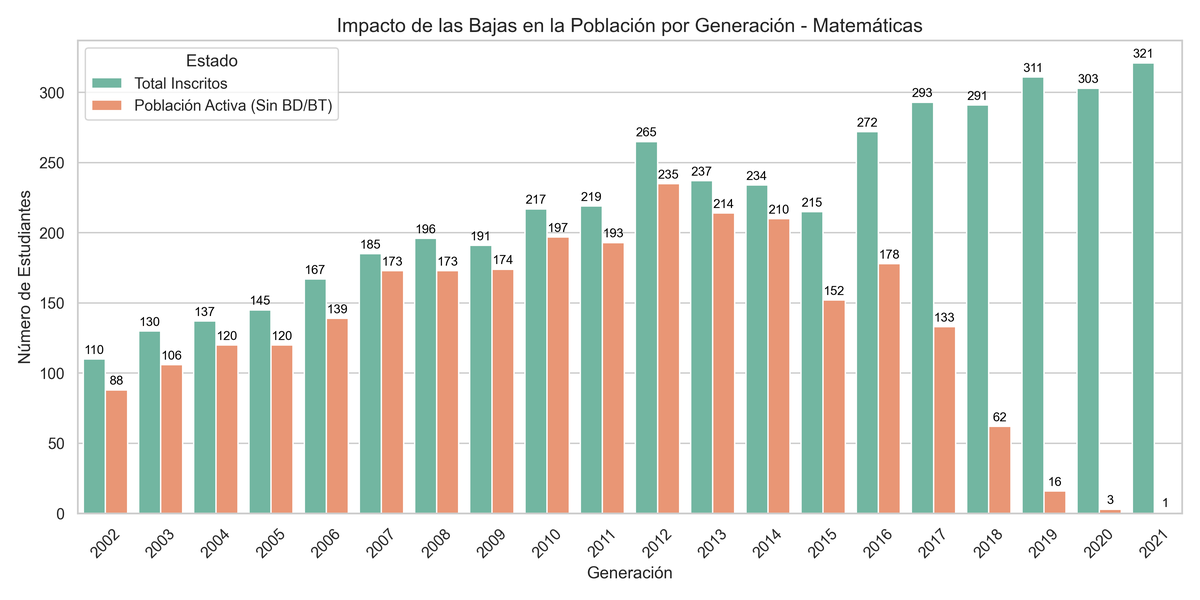
\includegraphics[width=0.8\textwidth]{poblacion_comparativa_matematicas}
    \caption{Comparativa de población estudiantil total vs. activa por generación (Matemáticas), ilustrando la atrición por bajas definitivas y temporales.}
    \label{fig:poblacion_matematicas}
\end{figure}

Esta atrición documentada resalta la importancia de aislar a los estudiantes activos para el modelado del rezago. Es sobre esta población residual —la cual permanece institucionalmente en curso o egresada— que surge el problema de la censura temporal en el semestre de término.

\subsection{Selección y depuración de variables}

Con fines analíticos, se eliminaron del conjunto de datos aquellas variables que no aportan
información relevante para el estudio de tendencias académicas, tales como el nombre del
estudiante y  el plan de estudios.

La variable \texttt{generación} se conservó en el conjunto de datos final, ya que permite
capturar posibles efectos de cohorte asociados a cambios institucionales, académicos o
contextuales entre distintos años de ingreso.

Asimismo, el análisis se restringió a los primeros ocho semestres de la trayectoria académica
(\texttt{s1} a \texttt{s8}). Esta decisión se fundamenta en que el rezago académico asociado a la
condición de Artículo 32 suele manifestarse a partir de etapas tempranas de la licenciatura y en
que los indicadores disponibles presentan mayor completitud y consistencia en dichos semestres.

\subsection{Integración de las fuentes de información}

Una vez depurados los datos, las cuatro hojas correspondientes a cada dimensión del Vector
Excalibur se integraron en un único conjunto de datos mediante una unión interna
(\textit{inner join}), utilizando la variable \texttt{Cuenta} como identificador.

Este procedimiento garantiza que el análisis se realice únicamente sobre estudiantes para los
cuales se dispone de información completa en las cuatro dimensiones consideradas, evitando la
introducción de valores faltantes estructurales derivados de la ausencia de alguna fuente de
información.

\section{Definición de la variable objetivo: semestre de término}

\subsection{Motivación}

Con el fin de estudiar el rezago académico desde una perspectiva cuantitativa, se definió una
variable objetivo que resume el momento en el que un estudiante concluye su licenciatura, o bien,
el punto a partir del cual su trayectoria académica se extiende más allá del tiempo
reglamentario.

Dicha variable permite transformar una trayectoria semestral completa en una medida resumida,
adecuada para su análisis mediante técnicas de estadística inferencial.

\subsection{Definición operativa}

La variable \texttt{semestre\_termino} se definió utilizando la hoja de \textit{Regularidad
gregoriana} del Vector Excalibur, de acuerdo con el siguiente criterio:

\begin{itemize}
    \item Para cada estudiante, se identifica el primer semestre mayor o igual a \texttt{s8} en
    el que el indicador de regularidad toma el valor igual a 1, lo cual se interpreta como la
    conclusión de la licenciatura bajo los criterios institucionales.
    \item En caso de que el estudiante no presente ningún valor igual a 1 a partir del semestre
    \texttt{s8}, se asigna el valor 20 a la variable \texttt{semestre\_termino}, indicando que la
    trayectoria académica se extiende hasta el máximo horizonte temporal considerado.
\end{itemize}

Formalmente, la variable se define como:

\[
\text{semestre\_termino}_i =
\begin{cases}
\min \{ k \geq 8 : s_k^{(i)} = 1 \}, & \text{si existe tal } k, \\
20, & \text{en otro caso}.
\end{cases}
\]

\subsection{Interpretación}

La variable \texttt{semestre\_termino} representa una aproximación cuantitativa al momento de
conclusión de la licenciatura y constituye la variable objetivo del estudio.

Valores pequeños de \texttt{semestre\_termino} indican trayectorias académicas más cortas,
mientras que valores grandes sugieren una mayor probabilidad de rezago académico y, en
particular, un mayor riesgo de encontrarse en condición de Artículo 32.

Esta variable permite vincular de manera directa los indicadores semestrales del Vector
Excalibur con el análisis de tendencias académicas mediante modelos estadísticos explicables.

\subsection{El problema de la censura por la derecha y el sesgo generacional}

La asignación artificial del valor 20 a los estudiantes que no han concluido su licenciatura (o que han desertado sin ser dados de baja oficialmente) introduce un desafío metodológico conocido en el análisis de supervivencia como \textit{censura por la derecha}.

Tratar un dato censurado como un valor numérico fijo ($k=20$) genera un sesgo significativo, pues aglomera de manera artificial una gran proporción de observaciones en la cota superior del tiempo reglamentario, creando una distribución fuertemente sesgada y bimodal. Esta concentración diluye la varianza de la muestra y atenúa las correlaciones paramétricas y no paramétricas.

Este problema es particularmente agudo al considerar el efecto generacional. Las cohortes de ingreso antiguas han tenido tiempo suficiente para alcanzar el semestre 20 (o titularse tardíamente), por lo que la proporción de datos censurados en dichas generaciones corresponde principalmente a casos de rezago extremo o abandono definitivo. En contraste, para las generaciones de ingreso recientes, una proporción considerable de la cohorte será clasificada con \texttt{semestre\_termino} $= 20$ simplemente porque, al momento de la observación, aún no ha transcurrido el tiempo necesario para que concluyan sus estudios de manera regular. 

Visualizar la distribución del semestre de término condicionada por la generación permite constatar empíricamente este sesgo: el promedio de la variable experimenta un repunte drástico en las cohortes recientes impulsado casi exclusivamente por la acumulación de datos censurados, lo que invalida el tratamiento de esta variable como puramente continua y advierte la necesidad de emplear técnicas de análisis multivariado o de supervivencia para mitigar este artefacto estadístico.

\begin{figure}[H]
    \centering
    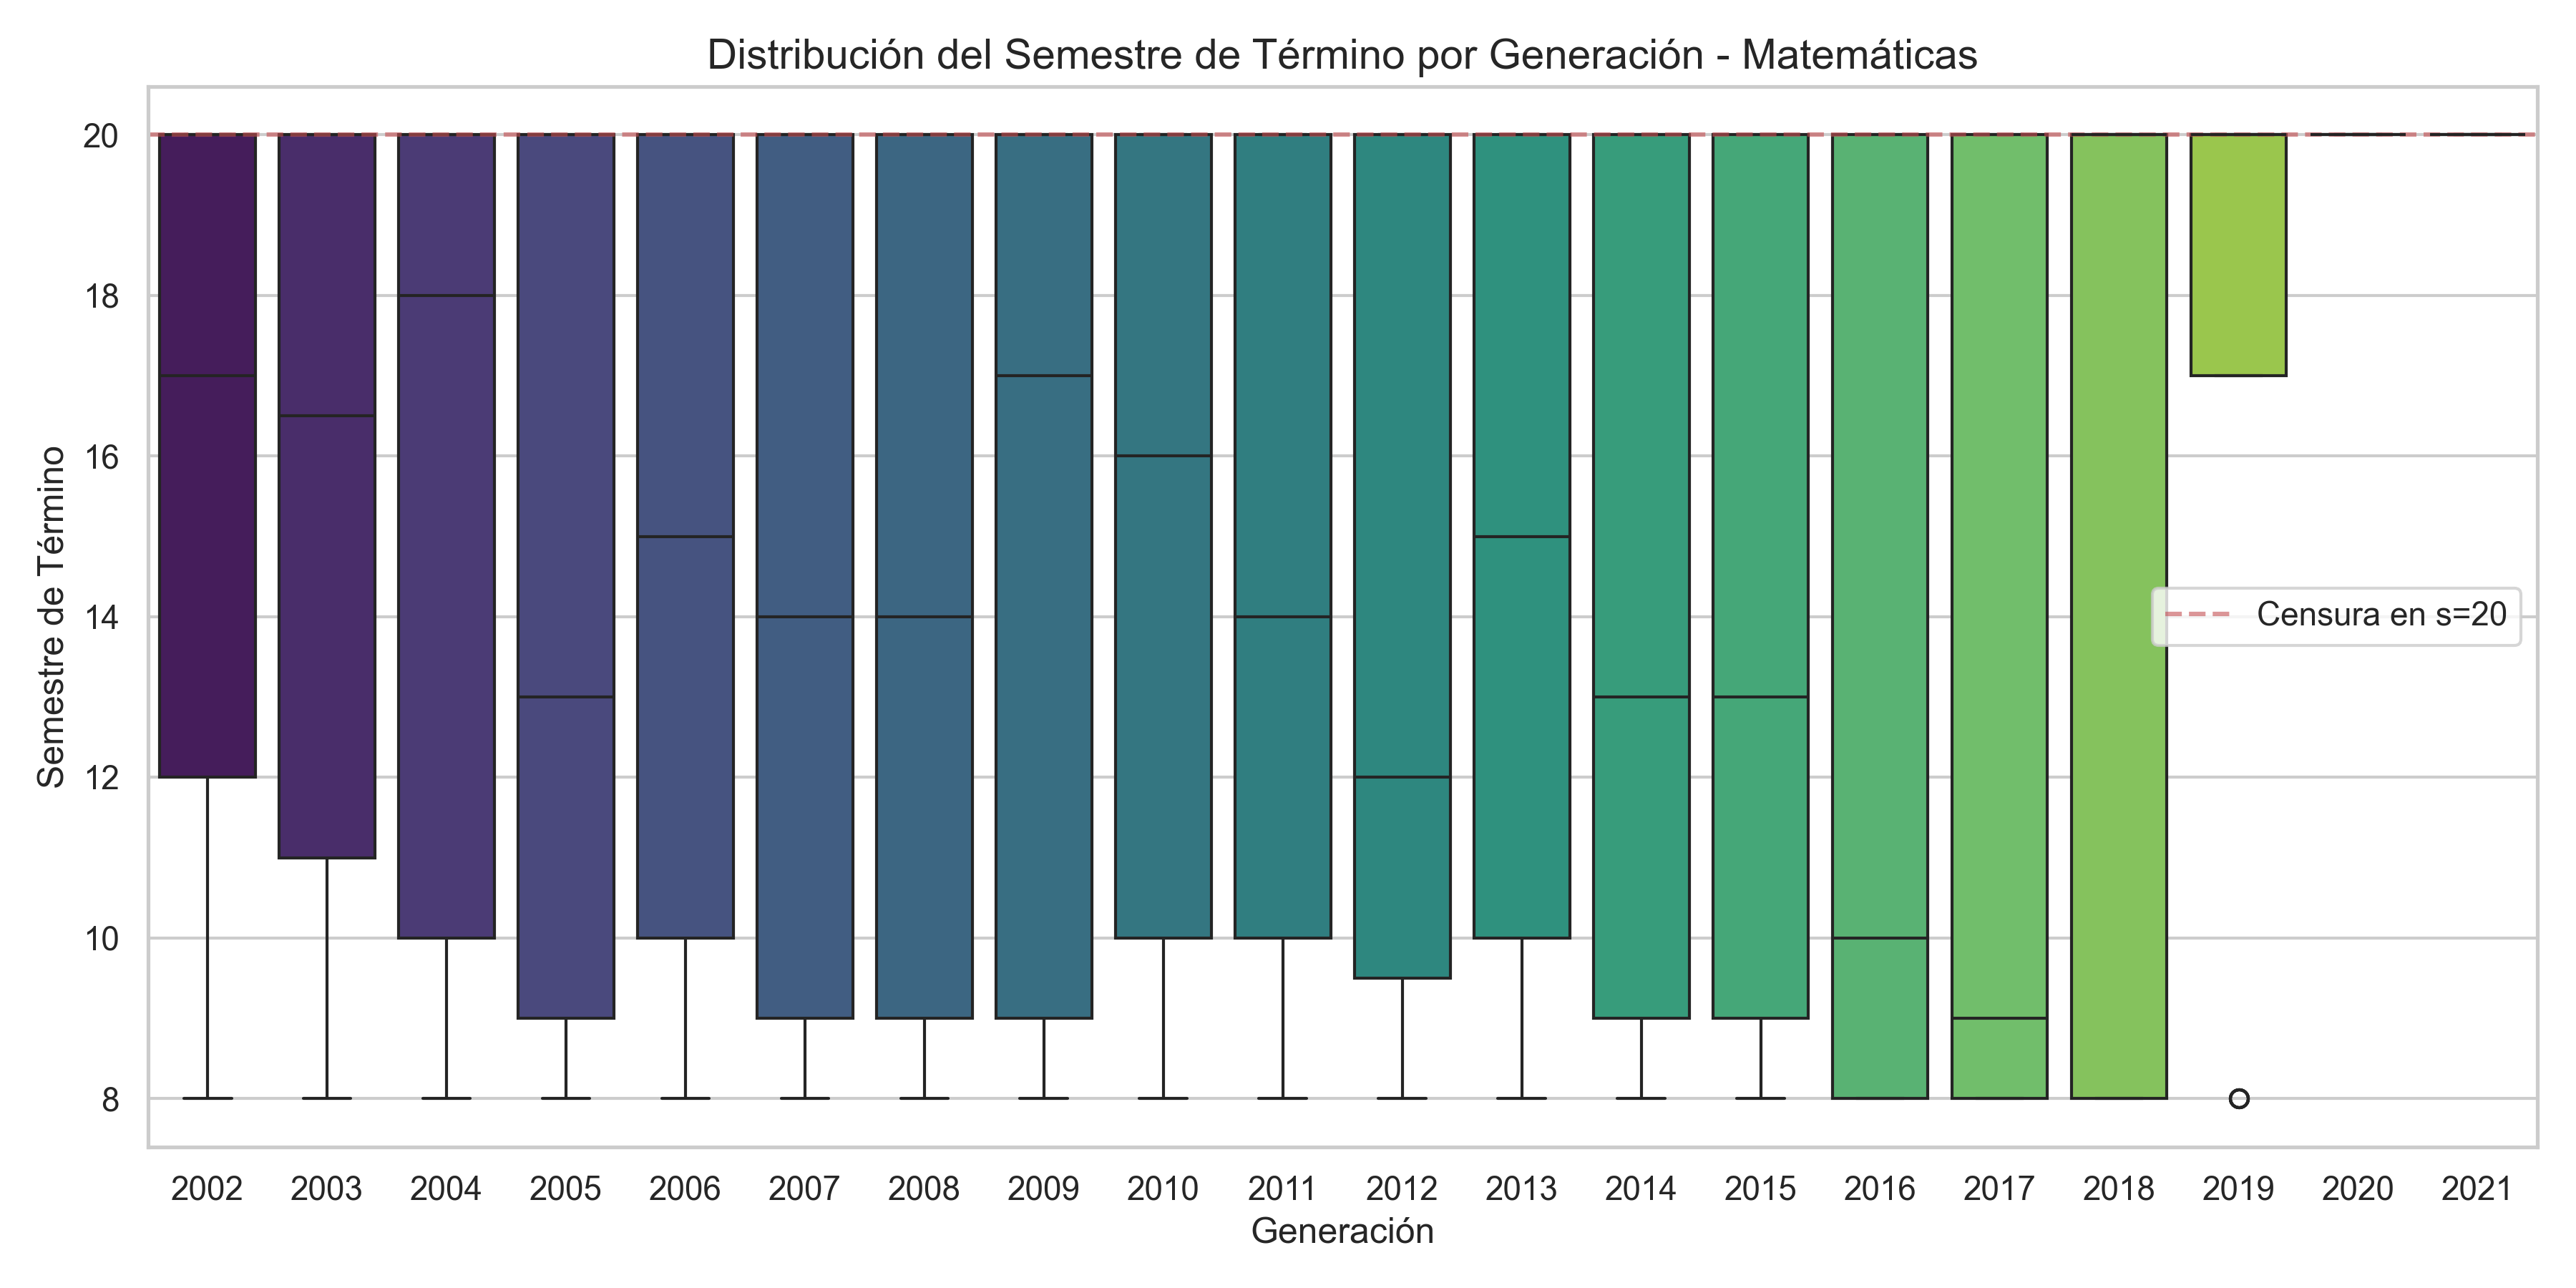
\includegraphics[width=0.8\textwidth]{boxplot_censura_gen_matematicas}
    \caption{Distribución del semestre de término por generación (Matemáticas), mostrando la acumulación artificial en $s=20$ para cohortes recientes.}
    \label{fig:boxplot_censura_matematicas}
\end{figure}

\subsection{Estrategias Analíticas Paralelas}

Para dar solución al problema de los riesgos competitivos (abandono vs. rezago continuo) y la censura por la derecha, la metodología de este estudio propone la construcción y análisis de tres conjuntos de datos paralelos:

\begin{enumerate}
    \item \textbf{Enfoque Base (Censurado):} Conserva la asignación de $k=20$ para los estudiantes que no han concluido. Se utiliza como línea base para dimensionar el impacto del sesgo metodológico.
    \item \textbf{Enfoque Truncado (A ciegas):} Restringe la muestra únicamente a las cohortes de ingreso anteriores a 2017 (Generación $\leq 2016$). En este conjunto, los estudiantes inconclusos se eliminan del análisis lineal (tratados como \textit{Missing Not At Random}), bajo el supuesto empírico de que la inmensa mayoría de los casos sin titular después de 16 semestres corresponden a abandono definitivo. Este enfoque permite correlacionar el rezago puramente en la población que sí logró culminar sus estudios.
    \item \textbf{Enfoque Multiclase (Informado):} Sustituye la predicción continua del semestre de término por la clasificación del estado final del estudiante. Se construyó una variable categórica evaluando tanto el tiempo de titulación como la caída del \textit{Índice de Esfuerzo} en los últimos semestres registrados, definiendo cuatro posibles estados: Titulado a tiempo ($k \leq 10$), Titulado con rezago ($10 < k < 20$), Abandono silencioso y Activo (aún cursando).
\end{enumerate}

Esta arquitectura de datos permite aislar los predictores del rezago académico (Enfoque Truncado) de los predictores del abandono escolar (Enfoque Multiclase), garantizando conclusiones estadísticamente robustas para cada fenómeno.

\subsection{Reincorporación de Bajas Temporales: Análisis de la Generación 2016}

A pesar de que el filtro inicial remueve el "ruido" de los abandonos, una revisión profunda del volumen de datos excluidos (Figura \ref{fig:poblacion_matematicas}) reveló un costo muestral inaceptable. Al analizar específicamente a la \textbf{Generación 2016} —elegida por ser la cohorte más moderna con tiempo suficiente para madurar sus procesos de titulación— se descubrió empíricamente que una fracción significativa de los alumnos con Baja Temporal (\textit{BT}) no abandona la carrera, sino que reingresa y concluye exitosamente sus estudios. 

Excluir de manera definitiva a la población con Baja Temporal significa descartar casos de éxito reales que experimentaron rezago justificado, lo cual atenta contra la representatividad estadística del modelo predictivo. Por tanto, surge el imperativo metodológico de reincorporar a estos estudiantes corrigiendo la distorsión que su periodo de ausencia genera sobre la variable \texttt{semestre\_termino}.

\begin{figure}[H]
    \centering
    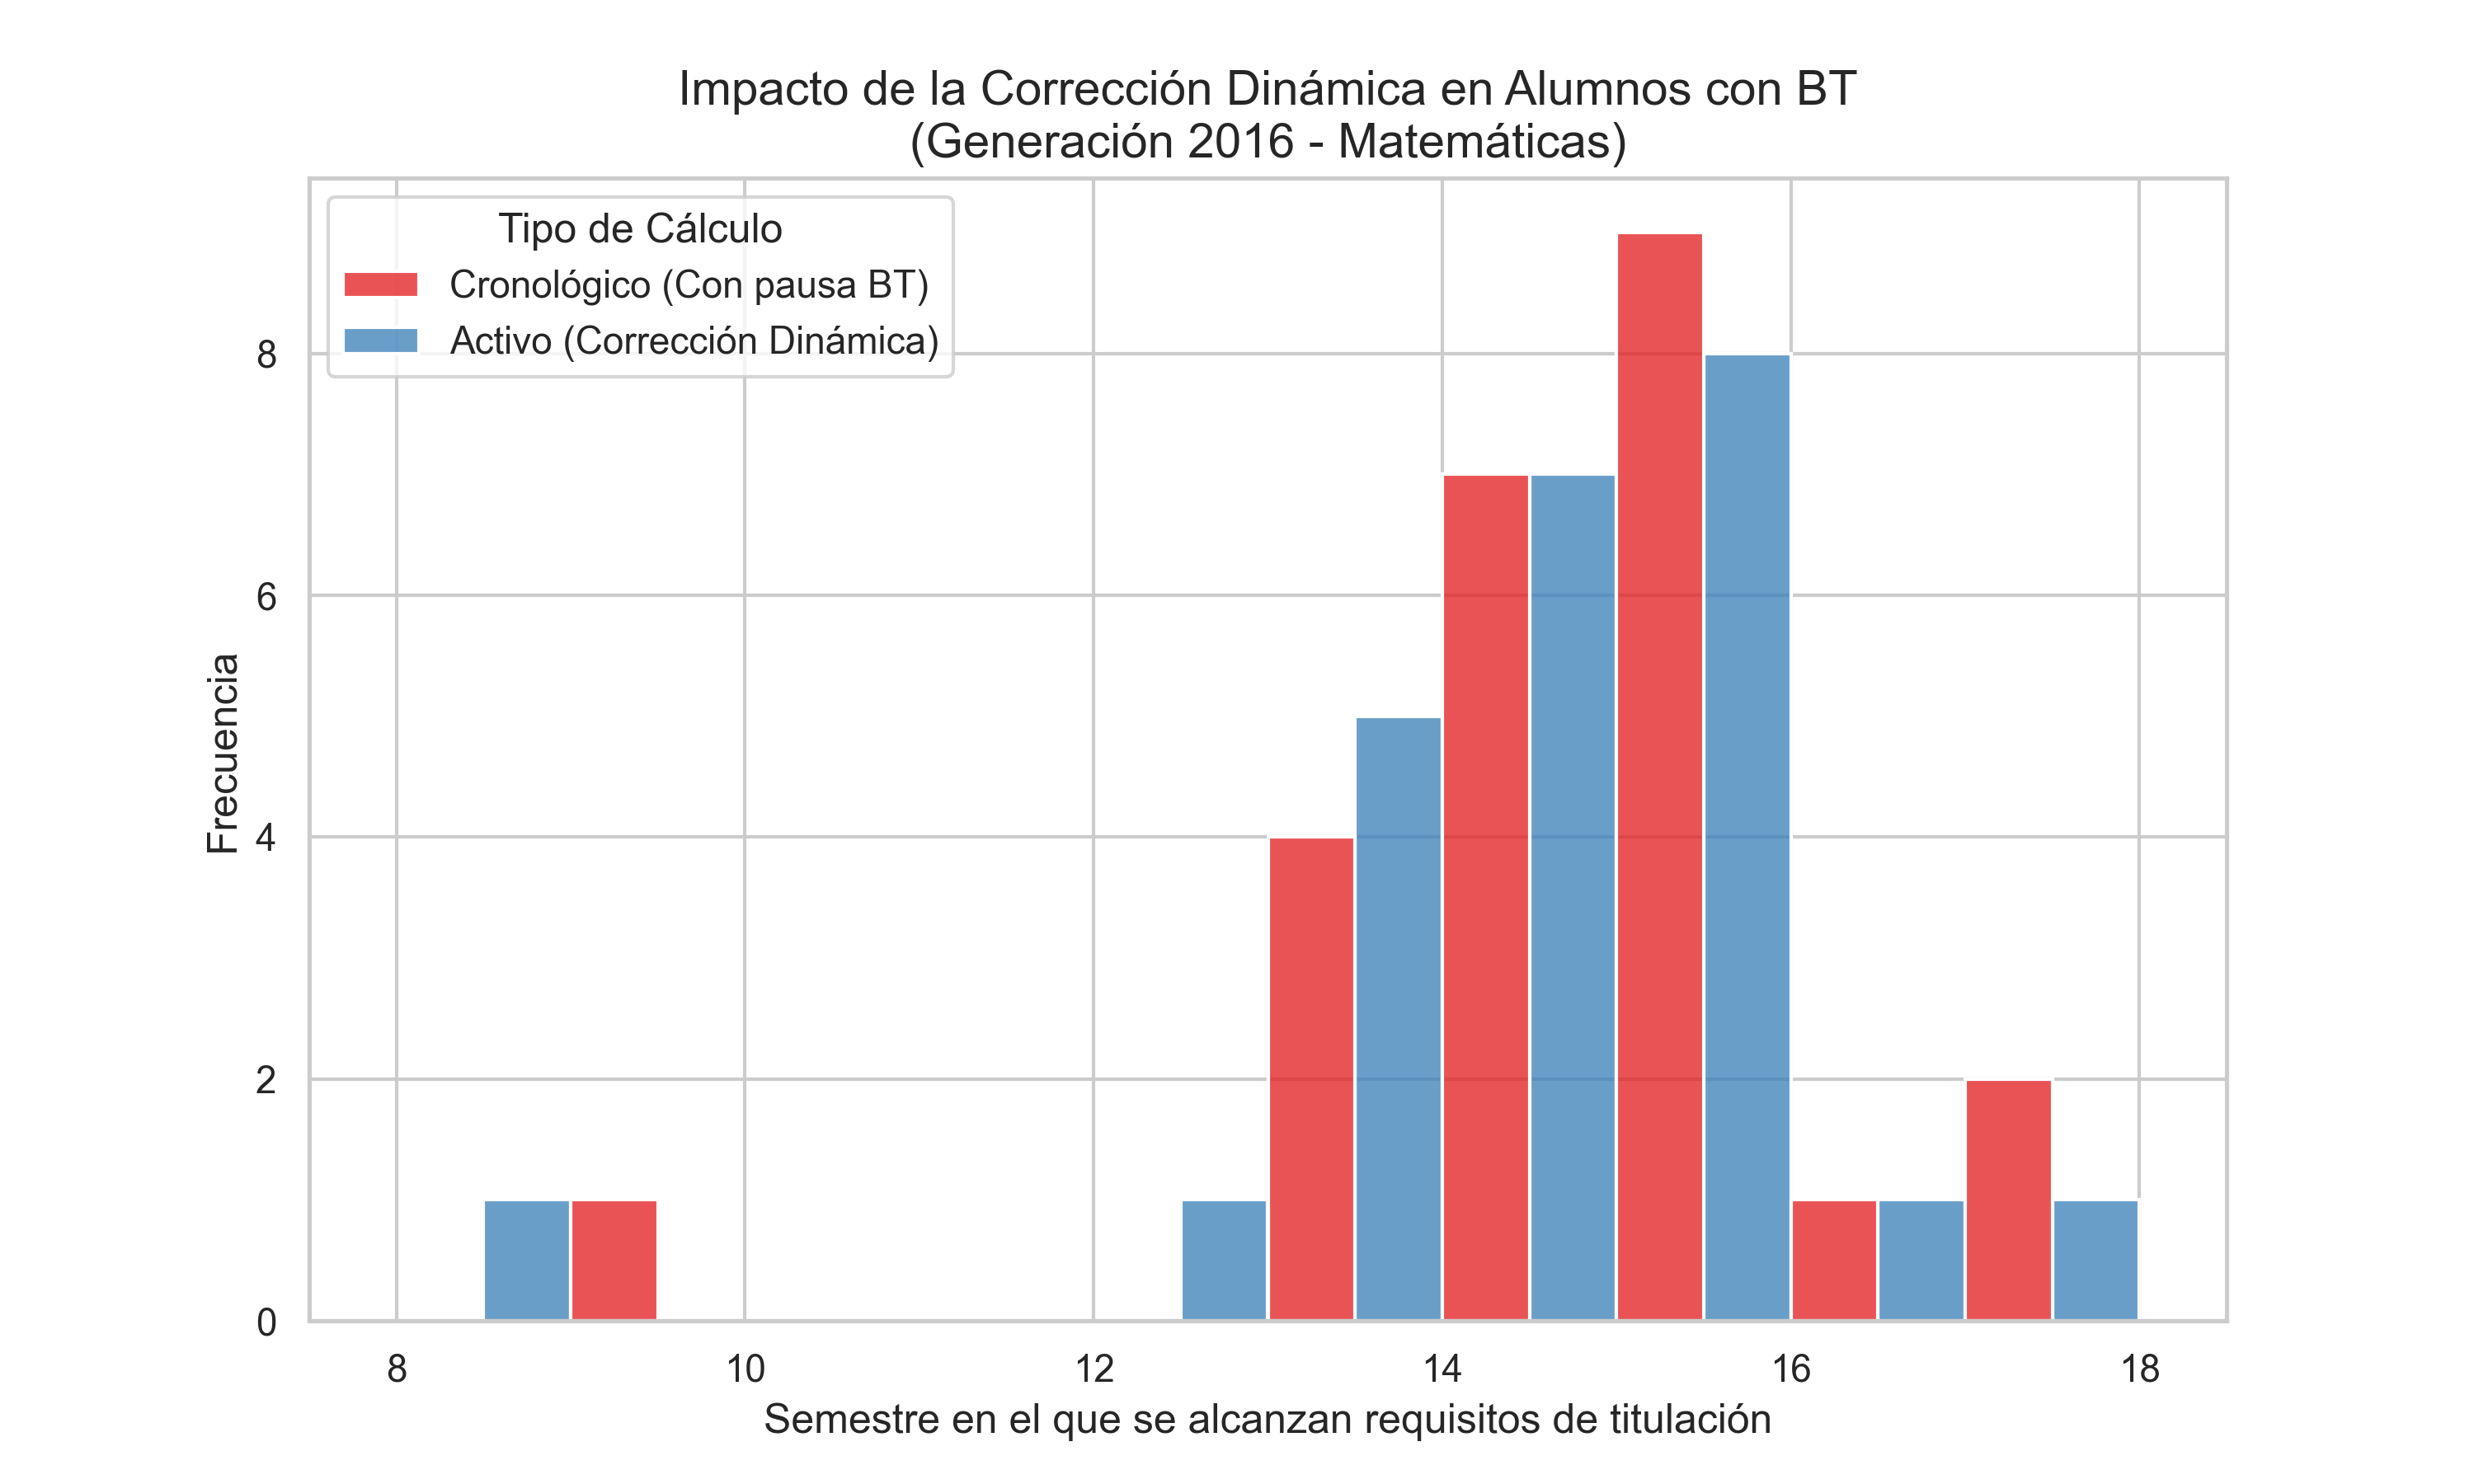
\includegraphics[width=0.8\textwidth]{correccion_bt_2016_matematicas}
    \caption{Distribución del semestre de término para alumnos de la Generación 2016 con Baja Temporal, contrastando el cálculo cronológico vs. corrección dinámica.}
    \label{fig:correccion_2016_matematicas}
\end{figure}

\subsection{Estrategias de Corrección: Fija vs. Dinámica}

Para evitar penalizar el rezago académico con periodos de ausencia administrativa, se evaluaron dos metodologías de ajuste temporal:

\subsubsection{Corrección Fija (Promedio de Ausencia)}
La primera aproximación consistió en calcular el promedio histórico de semestres inactivos para los estudiantes con \textit{BT} que logran titularse. Este enfoque resta una constante $C$ (el promedio de ausencia) al semestre de término cronológico de toda la subpoblación con Baja Temporal. Si bien es computacionalmente económica, esta técnica impone una homogeneidad irreal sobre un fenómeno altamente disperso.

\subsubsection{Corrección Dinámica (Transformación a Tiempo Activo)}
Para resolver la sobredispersión de la corrección fija, se implementó un algoritmo de compactación temporal individualizada que transforma el eje de \textit{Semestres Cronológicos} a \textit{Semestres Activos}. El procedimiento metodológico consiste en:
\begin{enumerate}
    \item \textbf{Detección de inactividad individual:} Se evaluó la variable \textit{Índice de Esfuerzo} de cada estudiante. Todo semestre con valor nulo se clasificó como inactivo.
    \item \textbf{Depuración de abandono prolongado:} Se excluyó permanentemente a cualquier estudiante con registro de Baja Definitiva o con un acumulado mayor a 4 semestres inactivos.
    \item \textbf{Compactación (Shift izquierdo):} Para cada alumno retenido, se eliminaron las columnas correspondientes a sus periodos inactivos y se recorrió su trayectoria hacia la izquierda, compactando sus verdaderos semestres de exposición académica.
    \item \textbf{Recálculo Dinámico:} Sobre esta nueva trayectoria compacta, se identificó el índice real activo en el que el estudiante alcanza las condiciones de egreso.
\end{enumerate}

\subsubsection{Análisis de Error}
Al comparar el desempeño de ambas estrategias, la Corrección Fija demostró ser insuficiente. Para la licenciatura en Matemáticas, aunque el promedio de semestres inactivos es relativamente bajo ($C=0.43$), el Error Absoluto Medio (MAE) de la Corrección Fija respecto a la trayectoria activa real fue de $0.62$ semestres, con desviaciones atípicas que alcanzaron un Error Máximo de $5.57$ semestres. En Física, la penalización máxima llegó a ser de $5.61$ semestres de error.

Estos resultados demuestran categóricamente que asumir un comportamiento de ausencia uniforme introduce un ruido estadístico severo en los extremos de la distribución. En consecuencia, se determinó utilizar la \textbf{Corrección Dinámica (Tiempo Activo)} como la transformación estándar para todo el proyecto, garantizando que los primeros 8 semestres de predicción reflejen puramente el desempeño del alumno mientras estuvo académicamente expuesto.

\end{document}
